\documentclass[11pt,a4paper]{article}
\usepackage[margin=2.2cm]{geometry}
\usepackage{fontspec}
\setmainfont{Times New Roman}
\setsansfont{Arial}
\setmonofont[Scale=0.85]{Consolas}
\usepackage{amsmath}
\usepackage{graphicx}
\usepackage{booktabs}
\usepackage{longtable}
\usepackage{pdflscape}
\usepackage{float}
\usepackage{caption}
\usepackage{enumitem}
\usepackage[hidelinks]{hyperref}
\captionsetup{font=small,labelfont=bf}
\setlist[itemize]{itemsep=2pt,topsep=4pt}
\setlength{\parskip}{5pt}
\setlength{\parindent}{0pt}
\graphicspath{{figures/}}

% one landscape page: the paper's figure beside ours
\newcommand{\comparison}[2]{%
  \begin{landscape}
  \section*{#2}
  \addcontentsline{toc}{subsection}{#2}
  \vspace{-3mm}
  \begin{minipage}[t]{0.495\linewidth}\centering
    {\small\textbf{Original}}\\[1mm]
    \includegraphics[width=\linewidth,height=0.83\textheight,keepaspectratio]{paper_#1.jpg}
  \end{minipage}\hfill
  \begin{minipage}[t]{0.495\linewidth}\centering
    {\small\textbf{Reproduced from the full 39-session run}}\\[1mm]
    \includegraphics[width=\linewidth,height=0.83\textheight,keepaspectratio]{ours_#1.png}
  \end{minipage}
  \end{landscape}
}

\title{\textbf{Distributed coding of choice, action and engagement across the mouse brain}\\[2mm]\large A figure-by-figure reproduction, with responses in VISp, LGd and LP}
\author{MohammadMahdi}
\date{November 2026}

\begin{document}
\maketitle

\begin{abstract}
This report reproduces the analyses of a brain-wide Neuropixels study of visual decisions in mice [1], from its public dataset [2], and redoes four of its plots for primary visual cortex (VISp) and two visual thalamic nuclei (LGd and LP). All 39 sessions were analysed: 9,538 trials and 29,178 neurons, of which 22,210 were assigned to the study's 42 regions. Each figure was then compared with the original panel by panel. The main results hold: action coding is global, visual coding follows a restricted pathway, choice coding is rare and localized, midbrain neurons prefer contralateral choices, and pre-stimulus engagement signals have opposite signs in neocortex and in subcortical regions. In VISp, LGd and LP, activity before the stimulus is lower in the task than in passive replay, and these regions carry visual and movement signals but very little choice coding. Some numbers differ from the paper, and those differences are listed.
\end{abstract}

\tableofcontents
\newpage

\section{Summary of the comparison}

Every panel group of Figures 1 to 5 and Extended Data Figures 1 to 9 was placed beside the original and rated. \textbf{Same} means the result cannot be told apart at reading accuracy. \textbf{Close} means the same pattern and conclusion, with small differences in values. \textbf{Partial} means the main conclusion holds but a difference is visible. \textbf{From the paper} marks a photo, histology image or cartoon with no data behind it: these are crops of the original figure, tagged ``from the paper'' in the figure itself.

\begin{table}[H]\centering\small
\begin{tabular}{@{}lrrrr@{}}
\toprule
Figure & Same & Close & Partial & From the paper \\
\midrule
Figure 1 & 0 & 4 & 1 & 5 \\
Figure 2 & 0 & 7 & 1 & 0 \\
Figure 3 & 1 & 6 & 0 & 0 \\
Figure 4 & 0 & 7 & 1 & 0 \\
Figure 5 & 0 & 5 & 1 & 0 \\
Extended Data Figure 1 & 1 & 5 & 1 & 0 \\
Extended Data Figure 2 & 0 & 2 & 0 & 3 \\
Extended Data Figure 3 & 0 & 0 & 0 & 1 \\
Extended Data Figure 4 & 0 & 3 & 1 & 0 \\
Extended Data Figure 5 & 0 & 6 & 1 & 1 \\
Extended Data Figure 6 & 0 & 2 & 0 & 0 \\
Extended Data Figure 7 & 0 & 6 & 0 & 0 \\
Extended Data Figure 8 & 0 & 3 & 2 & 0 \\
Extended Data Figure 9 & 0 & 6 & 1 & 0 \\
\midrule
Panel groups & 2 & 62 & 10 & 10 \\
\bottomrule
\end{tabular}

\caption{Agreement with the paper by figure. Ratings are by eye, supported by the numbers in Section~\ref{sec:numbers}.}
\end{table}

The ratings for the example neurons need care. Those neurons were chosen to resemble the paper's panels (Section~\ref{sec:neurons}), so their close match shows that such neurons exist in the data. It is not independent evidence for the paper's claims. The evidence is in the population panels, where nothing was selected.

The five largest differences from the paper are these:
\begin{enumerate}[itemsep=2pt]
\item \textbf{Fig 4c:} the time-by-group interaction is absent as in the paper (p = 1.0), but the group main effect is significant here (p = 7e-4). The paper reports none. So the conclusion that choice signals have the same timing across regions holds, while the claim of no group difference does not fully reproduce.
\item \textbf{Choice-selective neurons are fewer:} 79 in the midbrain and forebrain sets against the paper's 102, although the proportions preferring each side are close.
\item \textbf{Suppression of the non-preferred choice:} 16 of 46 midbrain neurons against 29 of 54. This is the largest proportional gap in the single-neuron results.
\item \textbf{Extended Data Table 1:} 23 of the 42 regions differ by more than 2\%, because the released region labels differ from those behind the paper's table.
\item \textbf{Fig 5d and Ext 7f:} the correlations are stronger than the paper's (r = 0.58 against 0.46, and 0.79 against 0.69).
\end{enumerate}

\section{Data and methods}

\subsection{Dataset}
The data are 39 sessions from 10 mice, recorded with Neuropixels probes in the left hemisphere [2]. On each trial, gratings of varying contrast could appear on the left, the right, both or neither, and mice turned a wheel to bring the higher-contrast grating to the center, or held still if there was none. Because all recordings are from the left hemisphere, \emph{contra} means the right stimulus and the Right choice. The sign conventions were checked against rewards in the data.

\subsection{Analysis}
The analysis was implemented in Python following the Methods of [1] and the authors' code [3].

\textbf{Trials.} Left and Right trials have a first movement of that kind 125 to 400 ms after the stimulus. For the regression, the authors' published trial lists were reproduced with no differences on all 39 sessions. For Fig 2d, f, h, Fig 5a, b and Ext 6b, trials were matched for contralateral contrast across correct contra, Miss and passive trials. This keeps 34 sessions, as in the paper.

\textbf{Neurons.} A neuron is a unit labelled good that fires at 0.1 sp/s or more from stimulus onset to 400 ms. Regions come from the Allen label at each neuron's peak channel, merged to the paper's 42 regions through the Allen hierarchy [4]. A region needs at least 13 neurons in a session and at least 2 mice.

\textbf{Firing rates.} Spikes were binned at 5 ms and smoothed with a causal half-Gaussian. For display, rates are smoothed with 20 ms, averaged over trials, and smoothed with 30 ms. Normalized rates are
\begin{equation}
r_{\text{norm}}(t) = \frac{r(t) - r_{\text{base}}}{r_{\text{base}} + 0.5}.
\end{equation}

\textbf{Kernel regression.} Each neuron's rate is modelled as a sum of kernels locked to stimuli and movements,
\begin{equation}
\hat f_n(t) = \sum_c \sum_{s \in S_c} K_{c,n}(t - s) + \sum_{m \in M} \big[ K_{m,n}(t - m) + D_m K_{D,n}(t - m) \big],
\end{equation}
with six Vision kernels, one Action kernel and one Choice kernel, giving 650 predictors. $D_m$ is +1 for Left (ipsi) and $-1$ for Right (contra), so a negative pre-movement Choice kernel means contra preference. A reduced-rank basis pooled over all sessions was fit with elastic net, copying the scaling of the software used in [1] and [5]: at $\alpha = 0.5$ the penalty is $\lambda_s = 0.5 / y_s$ for a neuron with rate s.d. $y_s$. A nested test measures what each kernel adds in cross-validation, with 2\% as the threshold.

\textbf{Other analyses.} Population decoding used L1 logistic regression on residuals. jPECC used 10 PCs and ridge CCA at each pair of times. Choice and detect probability combined Mann-Whitney statistics across the 16 stimulus conditions, with 2,000 shuffles. Engagement used a nested ANOVA on log rates from $-250$ to $-50$ ms, and an index from the task-passive rate difference from $-200$ to 0 ms.

\subsection{Figures}
The figures rebuild from saved results, with no new analysis. Colors were measured from the high-resolution figures embedded in the paper's PDF: region colors, line colors and all colormaps. Panels were placed at the pixel positions of the original.

Three plotting problems found during the comparison were corrected, and each changed a panel's appearance substantially:
\begin{itemize}
\item \textbf{Fig 2d-h and Ext 4b-e:} these now use the ``highly activated'' neurons of the Methods' section on visualizing firing rates. On all responsive neurons, the heatmaps were far too pale.
\item \textbf{Fig 4d and Ext 8:} the jPECC colormap had its black at $-0.1$, not 0, which turned zero correlation red.
\item \textbf{Ext 5c:} the legend reads L+R and L$-$R, so the plotted lines are twice each kernel.
\end{itemize}
Ext 1 was also found to use non-repeat trials. Using \texttt{repNum = 1} gives the paper's trial count exactly for 9 of 10 subjects.

\section{Assignment figures: VISp, LGd and LP}
\label{sec:assignment}

These figures redo Fig 2a-c, Fig 4e, Fig 5a and Ext 6b for the three regions, in the paper's style.

\begin{table}[H]\centering\footnotesize
\begin{tabular}{@{}lrrrrrrrrrr@{}}
\toprule
Region & Neurons & Sessions & Responsive & Regression & Pass 2\% & Vision & Action & Choice & T$-$P & G$-$M \\
\midrule
VISp & 917 & 12 & 616 & 708 & 259 & 208 & 16 & 1 & -0.68 & +0.02 \\
LGd & 789 & 8 & 362 & 481 & 33 & 4 & 11 & 0 & -1.67 & -0.36 \\
LP & 680 & 9 & 344 & 401 & 78 & 22 & 17 & 0 & -1.29 & -0.25 \\
\bottomrule
\end{tabular}

\caption{The three regions in the full run. Vision, Action and Choice count neurons passing the 2\% nested test. T$-$P is the pre-stimulus rate difference, task minus passive, and G$-$M is Go minus Miss, both in sp/s.}
\end{table}

\subsection{Fig 2a-c style: single-neuron rasters}
\begin{figure}[H]\centering
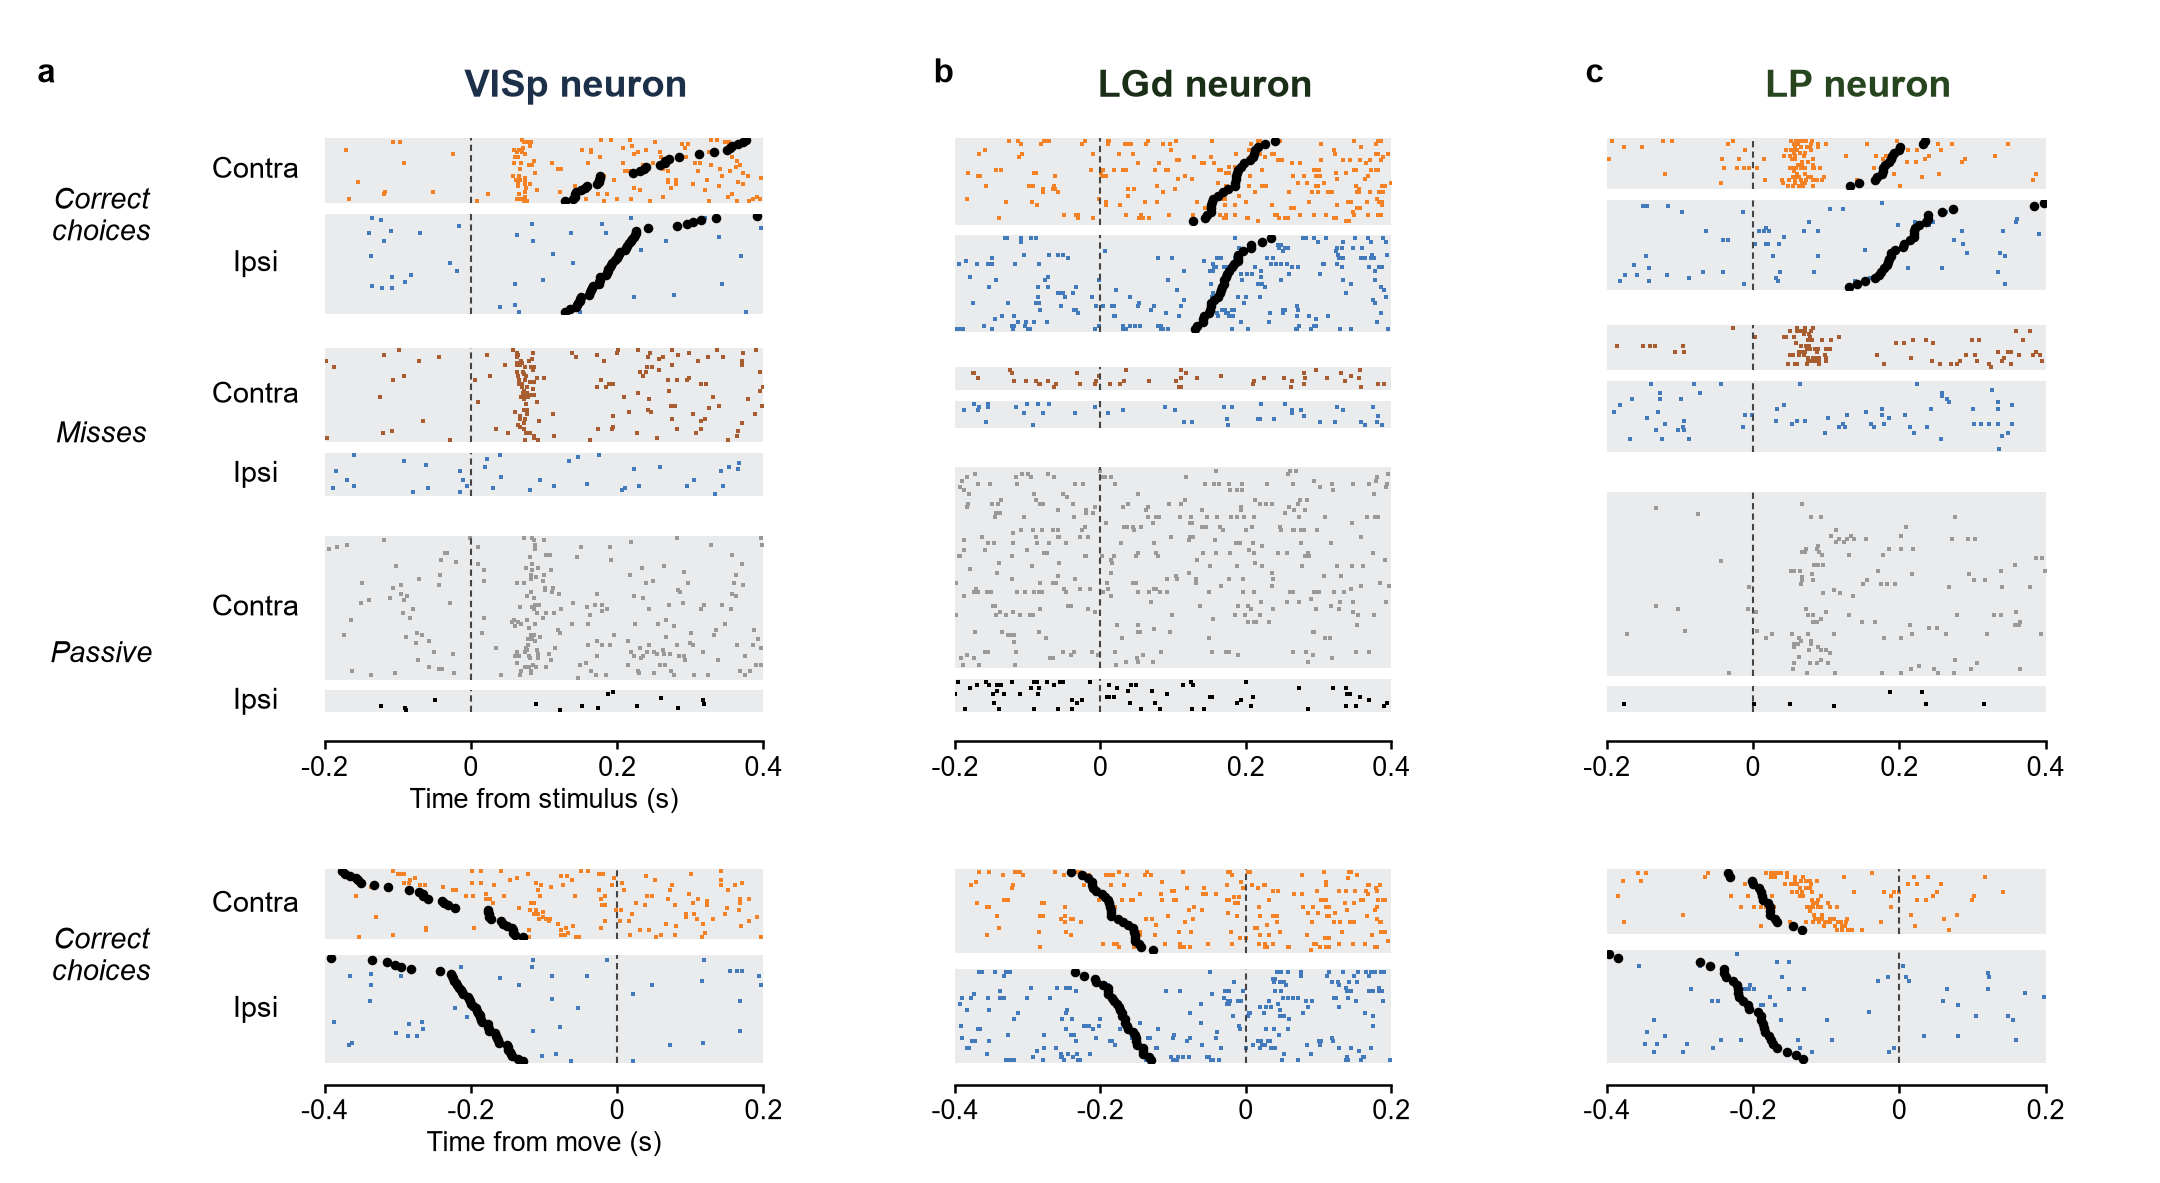
\includegraphics[width=0.92\linewidth]{assignment_fig2abc_rasters.png}
\caption{One neuron per region, on trials with a stimulus on one side only. Top six rows are aligned to the stimulus, with black dots marking movement. Bottom two rows are aligned to movement, with black dots marking the stimulus.}
\end{figure}
The VISp neuron fires a burst about 70 ms after a contralateral stimulus on correct, Miss and passive trials, and not after ipsilateral stimuli. The response is present with no movement at all, so it is visual. The LP neuron shows the same pattern. The LGd neuron is different: it fires at a high rate throughout, with little locked to the stimulus. This fits the paper's report that recorded LGd neurons had receptive fields away from the task stimuli [1].

\subsection{Fig 4e style: firing aligned to movement}
\begin{figure}[H]\centering
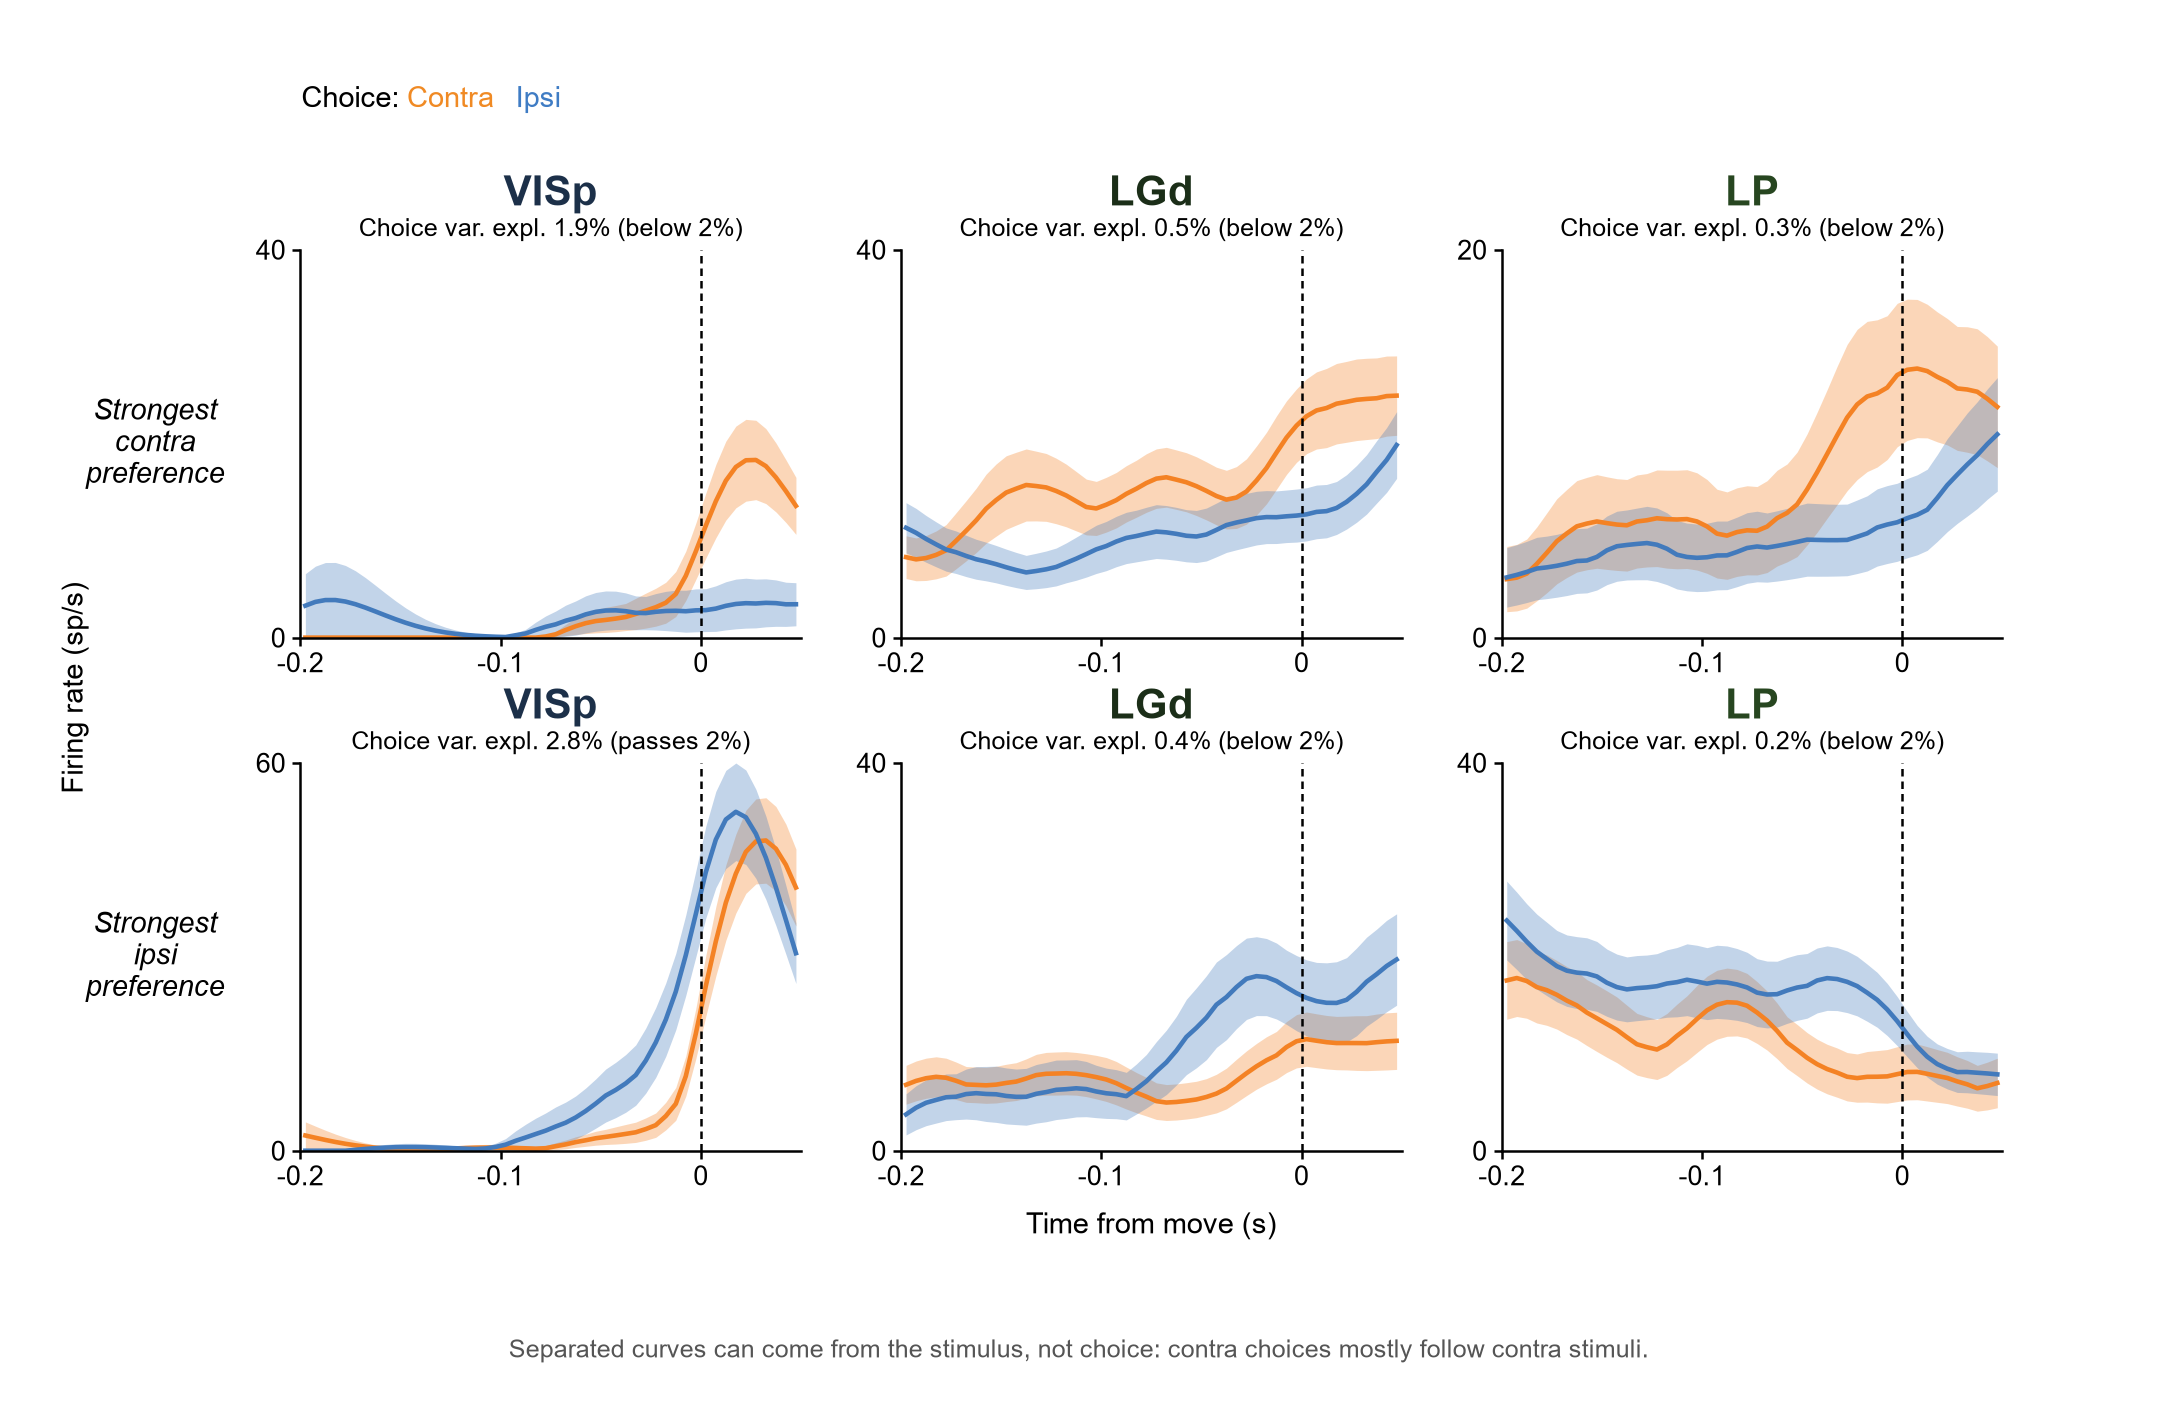
\includegraphics[width=0.9\linewidth]{assignment_fig4e_choice.png}
\caption{Rates aligned to movement, for contralateral (orange) and ipsilateral (blue) choices. Neurons have the highest nested Choice variance explained among those firing at 8 sp/s or more, in sessions with at least 15 trials per side.}
\end{figure}
Only one of the six neurons passes the 2\% Choice threshold: the VISp neuron in the bottom row, which is the single neuron of 708 in VISp to do so. No LGd or LP neuron passes. This agrees with the paper, which found no choice coding in VISp [1], and one neuron of the 259 tested (0.4\%) is no more than the 0.5\% false-positive rate of the shuffle test. Separated curves are therefore not evidence of choice coding here. Contra choices mostly follow contra stimuli, so a visual response alone can separate the two curves. The same caution applies to the VISp neuron in the paper's Fig 4a.

\subsection{Fig 5a style: Miss against Passive}
\begin{figure}[H]\centering
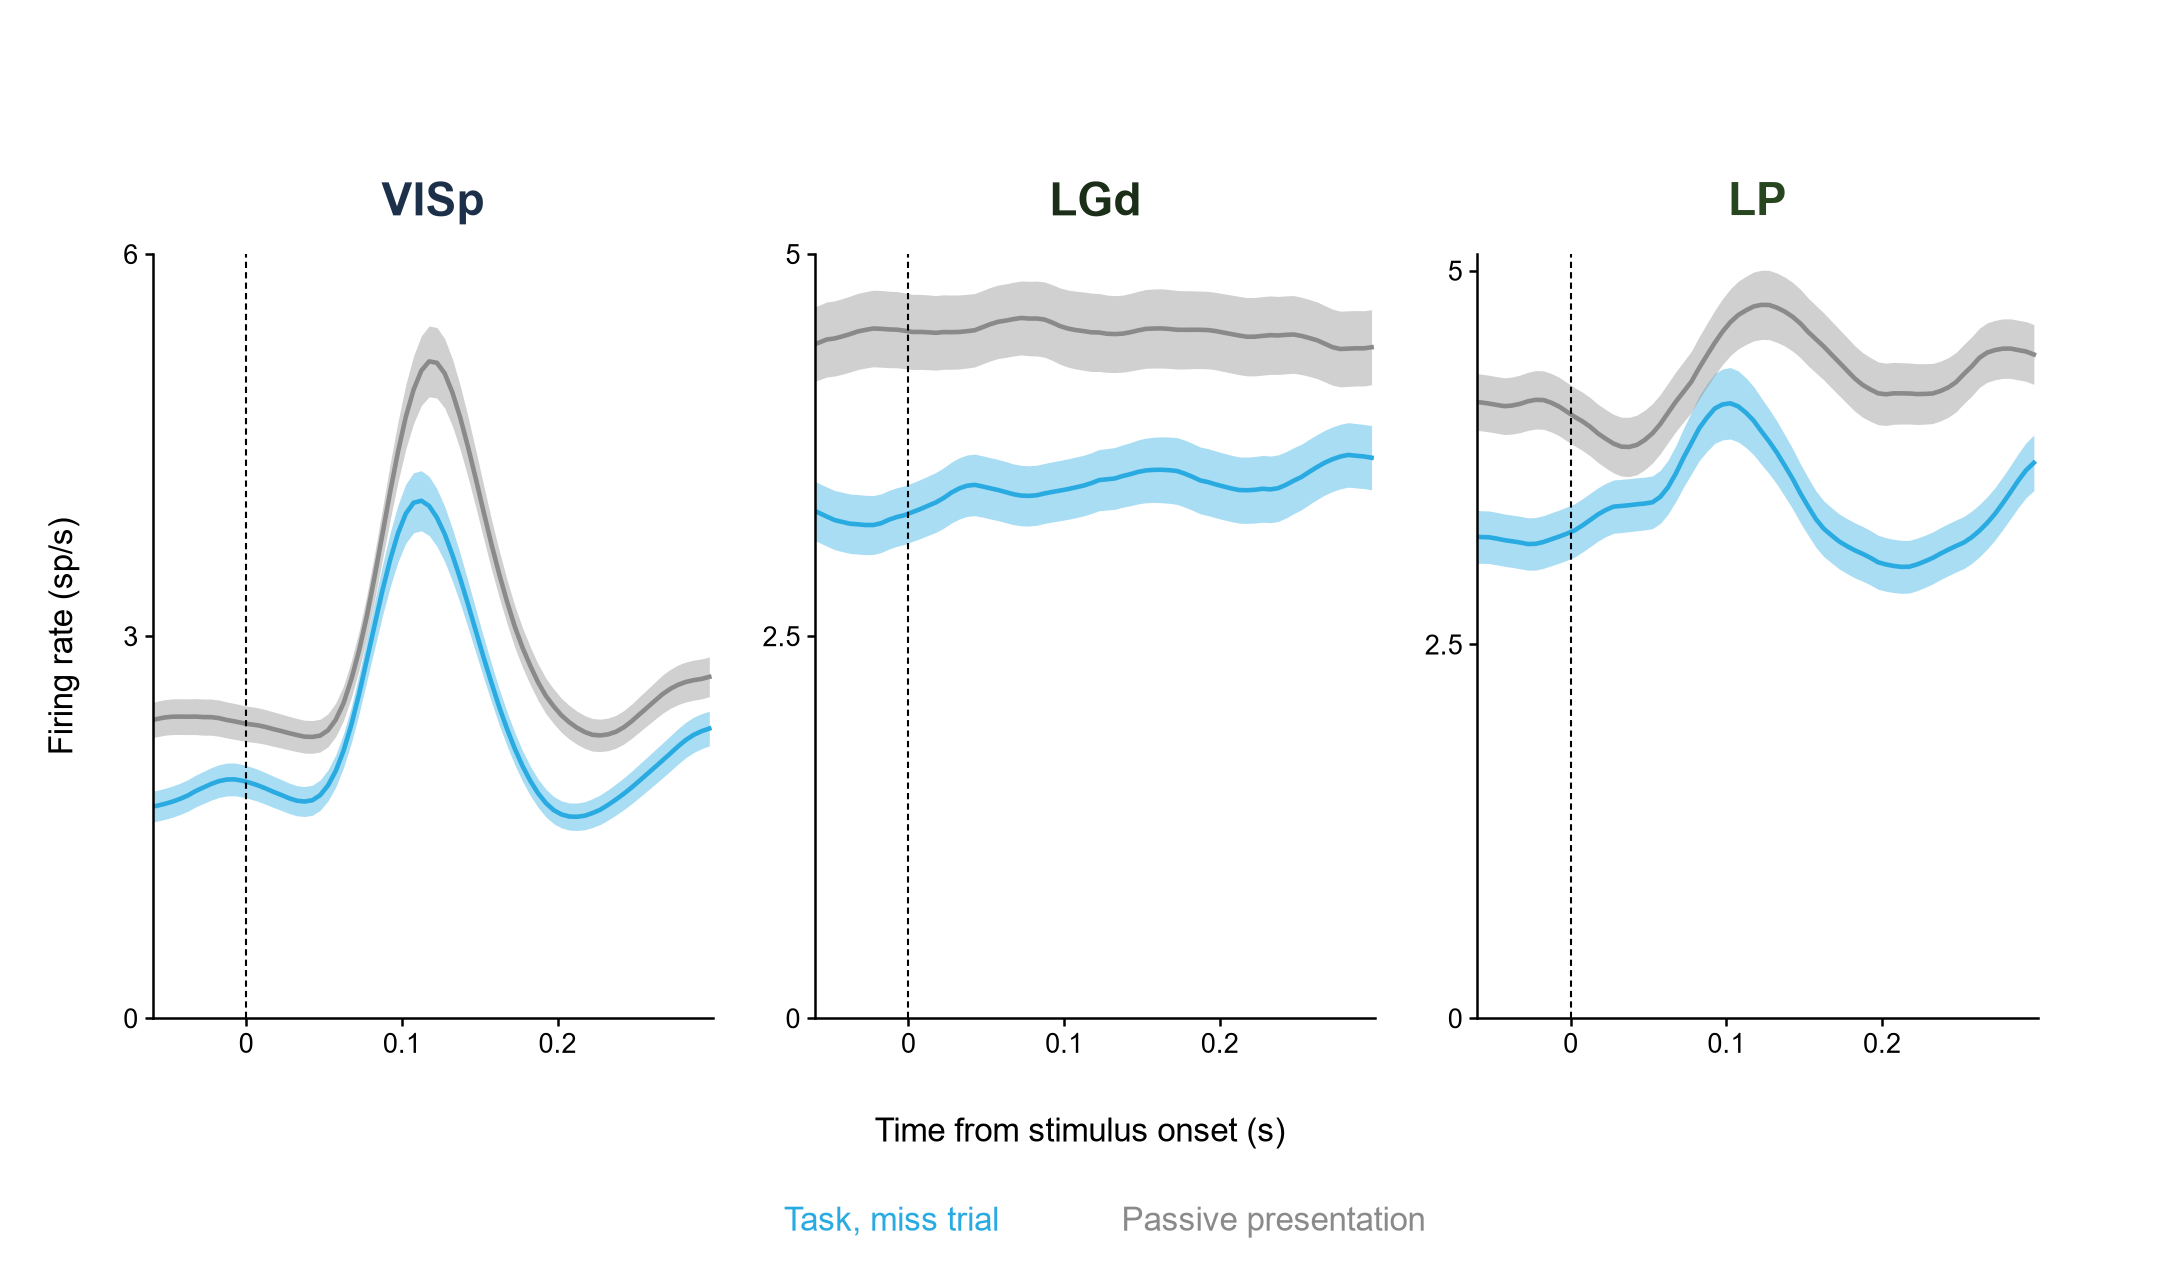
\includegraphics[width=0.9\linewidth]{assignment_fig5a_miss_passive.png}
\caption{Population average rate on Miss and passive trials with matched contralateral contrast. Shading is s.e.m. across neurons.}
\end{figure}
All three regions fire less before the stimulus in the task than in passive replay, by 0.68 sp/s in VISp, 1.67 in LGd and 1.29 in LP. The nested ANOVA finds this significant in all three. The paper reports the same direction for neocortex and visual thalamus [1]. VISp also shows the visual response after the stimulus, with a similar shape in the two conditions.

\subsection{Ext 6b style: Go, Miss and Passive}
\begin{figure}[H]\centering
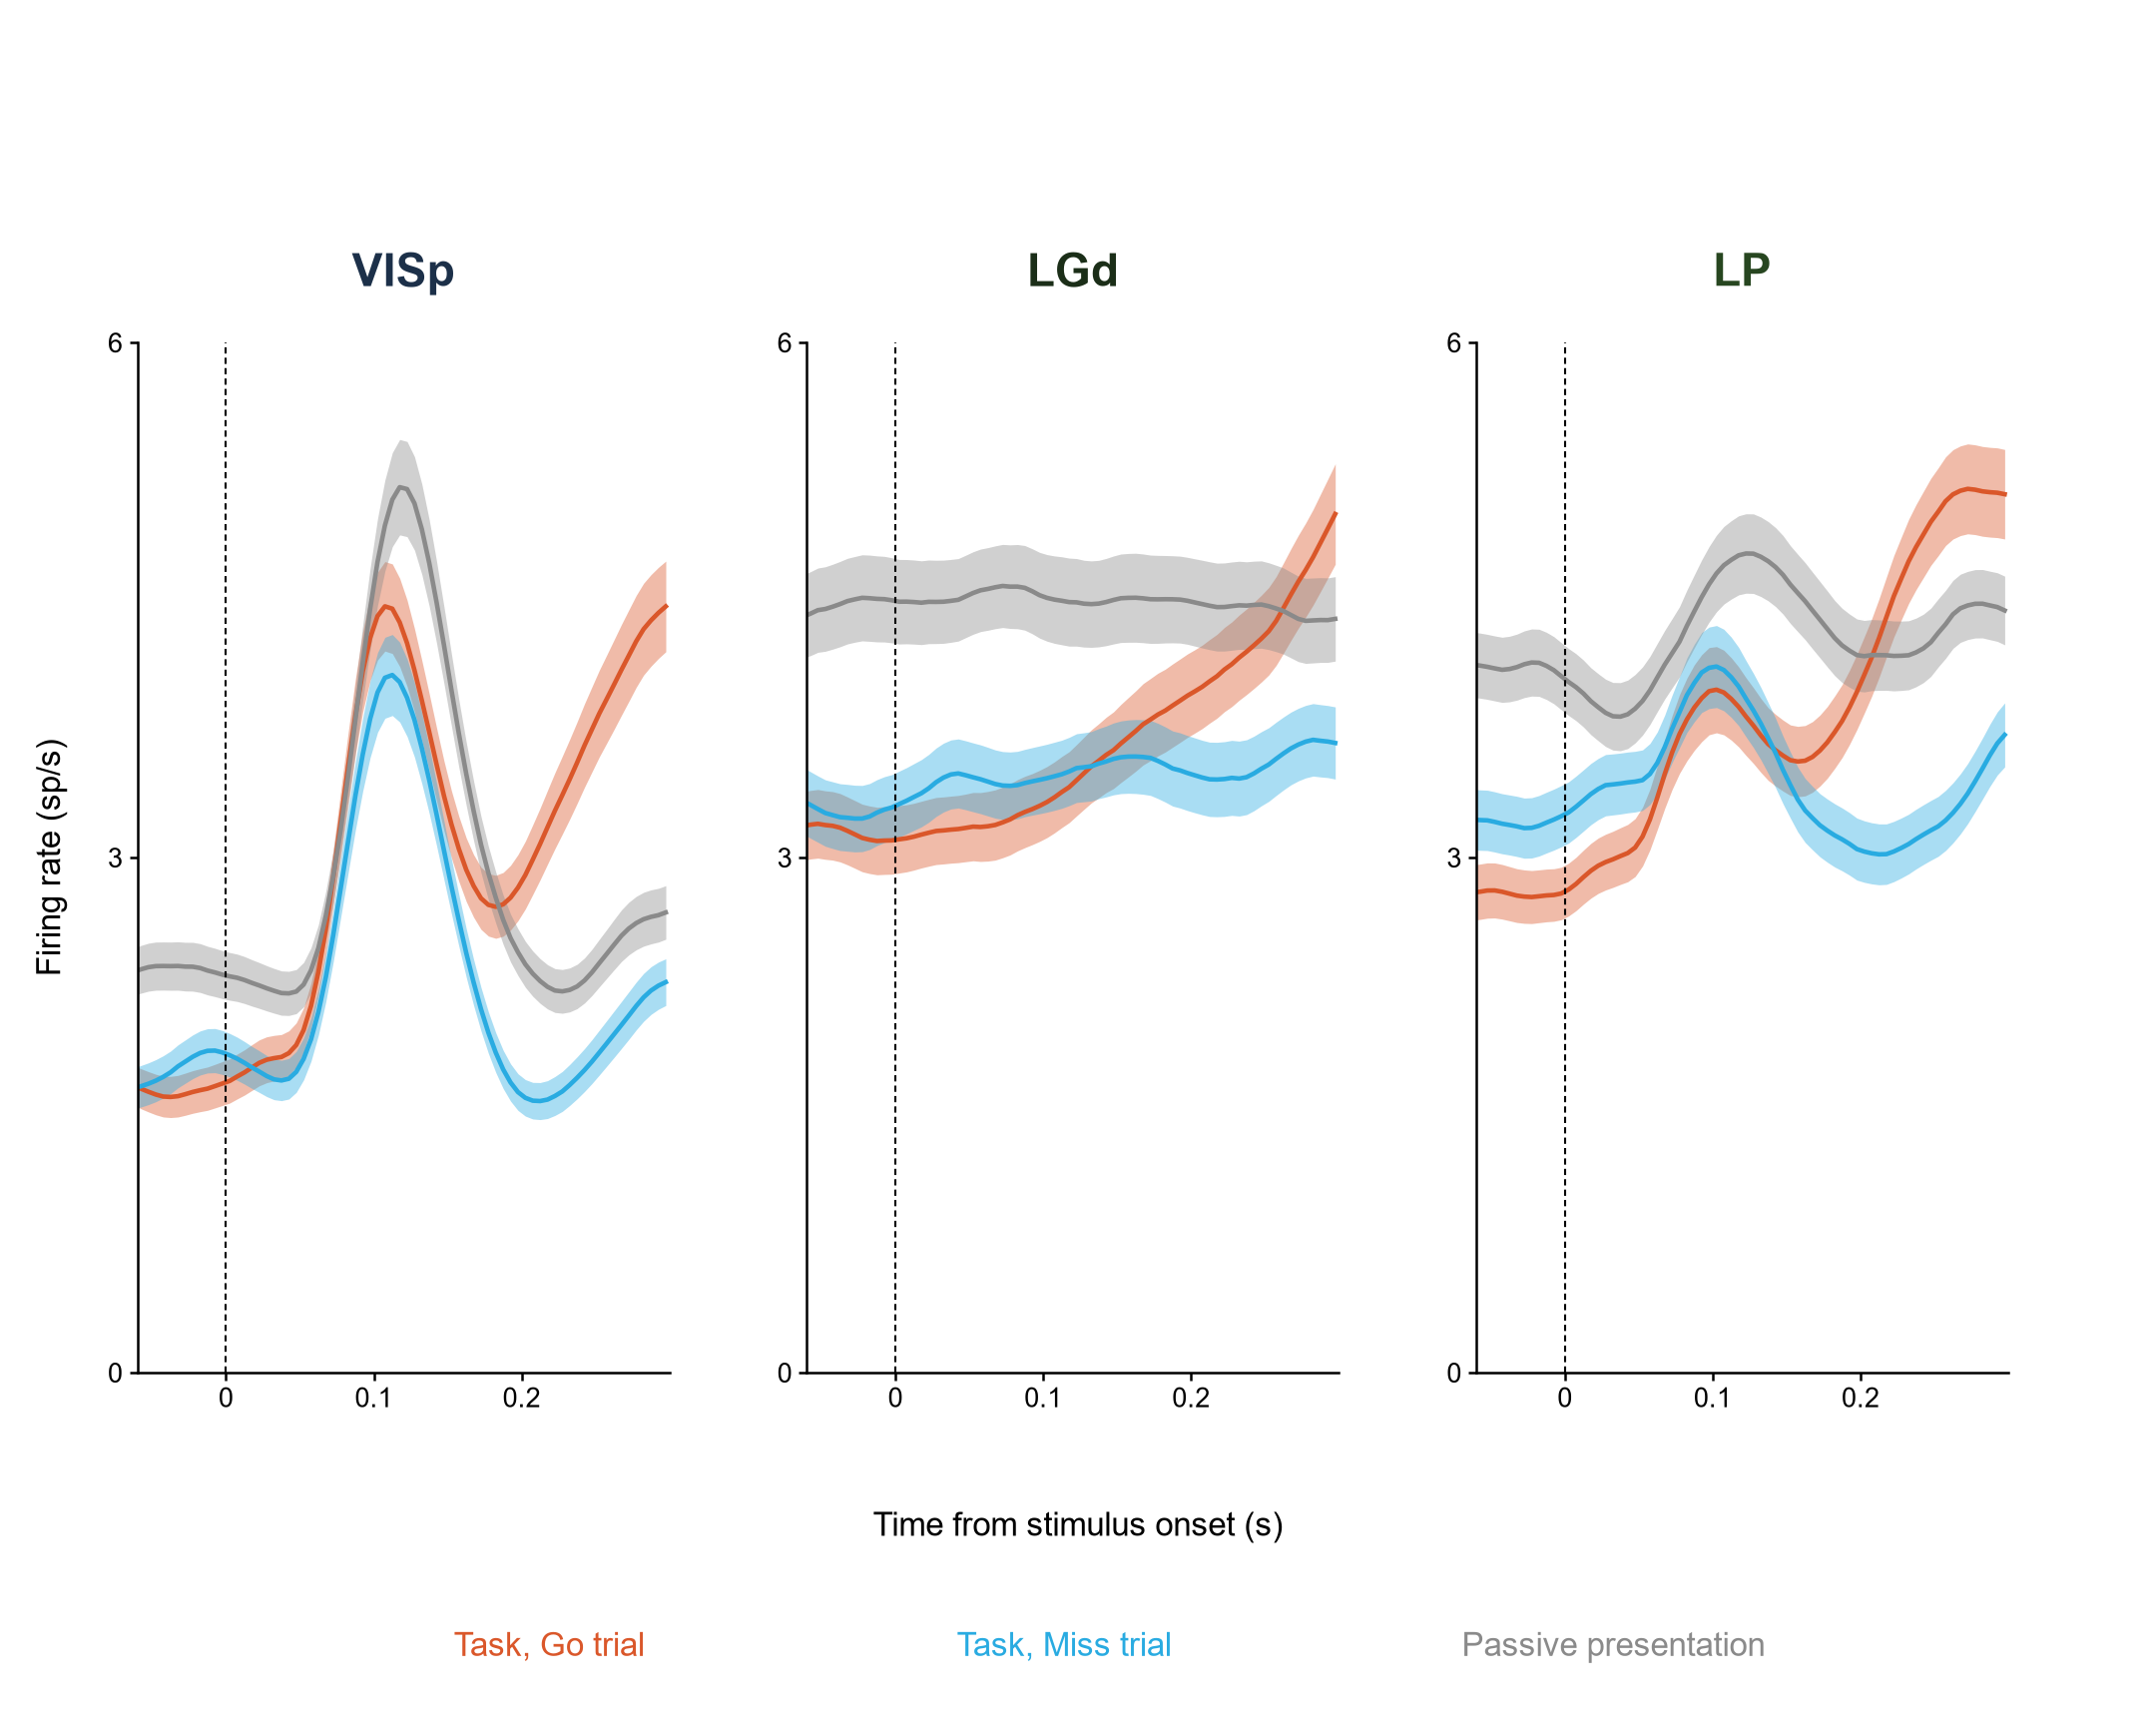
\includegraphics[width=0.9\linewidth]{assignment_ext6b_go_miss_passive.png}
\caption{Population average rate on Go, Miss and passive trials with matched contralateral contrast.}
\end{figure}
Before the stimulus, the order is Passive above Miss and Go in all three regions, which is the pattern the paper describes for these regions [1]. Go and Miss are close before the stimulus in VISp, and Go is a little below Miss in LGd and LP. After about 150 ms the Go trace rises, reflecting movement.

\subsection{Neurons shown}
\begin{table}[H]\centering\footnotesize
\begin{tabular}{@{}llp{5.2cm}rr@{}}
\toprule
Region & Panel & Session & Cluster & Choice var. expl. \\
\midrule
VISp & Raster & \texttt{Muller\_2017-01-07} & 683 & - \\
VISp & Contra preference & \texttt{Forssmann\_2017-11-01} & 268 & 1.9\% \\
VISp & Ipsi preference & \texttt{Cori\_2016-12-18} & 798 & 2.8\% \\
LGd & Raster & \texttt{Lederberg\_2017-12-09} & 454 & - \\
LGd & Contra preference & \texttt{Lederberg\_2017-12-09} & 454 & 0.5\% \\
LGd & Ipsi preference & \texttt{Forssmann\_2017-11-01} & 534 & 0.4\% \\
LP & Raster & \texttt{Hench\_2017-06-15} & 1244 & - \\
LP & Contra preference & \texttt{Moniz\_2017-05-15} & 179 & 0.3\% \\
LP & Ipsi preference & \texttt{Moniz\_2017-05-15} & 235 & 0.2\% \\
\bottomrule
\end{tabular}

\caption{Neurons in the assignment figures. Raster neurons have the most reliable contralateral stimulus response in a session with at least 15 correct trials per side.}
\end{table}

\section{Example neurons}
\label{sec:neurons}

The paper does not identify its example neurons. To get as close as the data allow, the curves in each example panel were digitized from the paper's high-resolution figures, and every neuron in that region was scored against them in sp/s. Candidates had to pass the test their panel implies: a neuron shown as choice-selective must pass the nested Choice test, and a neuron shown with no visual response must not pass the Vision test. For Fig 2, row heights also count, because they follow each session's trial counts.

\textbf{Curve error} is the root-mean-square difference from the paper's curves, as a percentage of the panel's peak. The chosen neurons are close matches, and they need not be the same cells. One result stands out: for the VISpm neuron of Fig 2b, curves and row heights separately pointed to \texttt{Cori\_2016-12-17}, so that may be the paper's own session.

\begin{longtable}{@{}p{3.6cm}p{1.5cm}p{5.4cm}p{1.4cm}p{2cm}@{}}
\toprule
Panel & Region & Session & Cluster & Curve error \\
\midrule
\endhead
Fig 2a, 3b & SUB & \texttt{Hench\_2017-06-15} & 1205 & 30\% \\
Fig 2b, 3a & VISpm & \texttt{Cori\_2016-12-17} & 1145 & 16\% \\
Fig 2c, 4a (ZI) & ZI & \texttt{Richards\_2017-11-01} & 791 & 9\% \\
Fig 4a VISp & VISp & \texttt{Cori\_2016-12-18} & 647 & 15\% \\
Fig 4a MRN & MRN & \texttt{Radnitz\_2017-01-11} & 420 & 10\% \\
Fig 4a CP & CP & \texttt{Radnitz\_2017-01-12} & 1105 & 6\% \\
Ext 4a VISp & VISp & \texttt{Moniz\_2017-05-16} & 1096 & 4\% \\
Ext 4a VISam & VISam & \texttt{Muller\_2017-01-08} & 605 & 13\% \\
Ext 5a, c & APN & \texttt{Moniz\_2017-05-15} & 669 & 19\% \\
Fig 4e panel 1 & MRN & \texttt{Muller\_2017-01-07} & 969 & 24\% \\
Fig 4e panel 2 & MRN & \texttt{Radnitz\_2017-01-11} & 426 & 14\% \\
Fig 4e panel 3 & SCm & \texttt{Tatum\_2017-12-07} & 665 & 5\% \\
Fig 4e panel 4 & SCm & \texttt{Lederberg\_2017-12-07} & 820 & 4\% \\
Fig 4e panel 5 & MOs & \texttt{Muller\_2017-01-07} & 423 & 21\% \\
Fig 4e panel 6 & MOs & \texttt{Radnitz\_2017-01-08} & 467 & 6\% \\
Fig 4e panel 7 & CP & \texttt{Richards\_2017-11-01} & 302 & 26\% \\
Fig 4e panel 8 & CP & \texttt{Hench\_2017-06-18} & 440 & 17\% \\
\bottomrule
\end{longtable}


The top five candidates for each panel are in \texttt{analysis/results/example\_scores.csv}.

\section{Comparison with the paper's numbers}
\label{sec:numbers}

\begin{longtable}{@{}p{8.2cm}p{3.2cm}p{3.9cm}@{}}
\toprule
Quantity & Paper & Full run \\
\midrule
\endhead
Neurons & 29134 & 29178 \\
Localized neurons & 22458 & 22210 \\
Modulated neurons & 13,466 (60.0\%) & 12,972 (58.4\%) \\
Sessions with contrast-matched trials & 34 of 39 & 34 of 39 \\
Sessions in CP analysis & 33 of 39 & 33 of 39 \\
Sessions in DP analysis & not stated & 39 of 39 \\
Shuffle false positives & 0.33\% & 0.50\% \\
Midbrain choice neurons preferring contra & 53/54 & 45/46 \\
Midbrain suppressed for non-preferred choice & 29/54 & 16/46 \\
Forebrain choice neurons preferring ipsi & 19/48 & 11/33 \\
Forebrain suppressed for non-preferred choice & 10/48 & 6/33 \\
Focality: action, contra vision, choice & 0.040, 0.069, 0.079 & 0.040, 0.065, 0.071 \\
Fig 5d correlation & r = 0.46, p = 0.002 & r = 0.58, p = 6.33e-05 \\
Mean engagement index difference & 8.42 & 9.15 (n = 34) \\
Ext 7f with Go-Miss, DP-qualified sessions (39) & r = 0.69 & r = 0.79 \\
Ext 7f with Task-Passive, DP-qualified sessions & r = 0.48 & r = 0.50 \\
Ext 7f with Go-Miss, 33-session CP subset sessions (33) & r = 0.69 & r = 0.81 \\
Ext 7f with Task-Passive, 33-session CP subset sessions & r = 0.48 & r = 0.47 \\
\bottomrule
\end{longtable}


Exact equality is not expected for results that depend on random splits, or on a different solver from the original.

\begin{table}[H]\centering\scriptsize
\begin{tabular}{@{}lrrr@{\hspace{6mm}}lrrr@{\hspace{6mm}}lrrr@{}}
\toprule
Region & Paper & Ours & \% & Region & Paper & Ours & \% & Region & Paper & Ours & \% \\
\midrule
ACA & 608 & 651 & +7.1 & MD & 381 & 388 & +1.8 & SCm & 997 & 992 & -0.5 \\
ACB & 255 & 261 & +2.4 & MG & 276 & 284 & +2.9 & SCs & 317 & 281 & -11.4 \\
APN & 235 & 236 & +0.4 & MOp & 682 & 680 & -0.3 & SNr & 274 & 273 & -0.4 \\
BLA & 261 & 266 & +1.9 & MOs & 1534 & 1335 & -13.0 & SSp & 461 & 448 & -2.8 \\
CA1 & 1129 & 1150 & +1.9 & MRN & 857 & 875 & +2.1 & SUB & 669 & 661 & -1.2 \\
CA3 & 438 & 430 & -1.8 & OLF & 684 & 695 & +1.6 & VISa & 285 & 288 & +1.1 \\
CP & 914 & 910 & -0.4 & ORB & 770 & 789 & +2.5 & VISam & 805 & 804 & -0.1 \\
DG & 711 & 702 & -1.3 & PAG & 130 & 128 & -1.5 & VISl & 403 & 382 & -5.2 \\
GPe & 274 & 281 & +2.6 & PL & 728 & 730 & +0.3 & VISp & 923 & 917 & -0.7 \\
ILA & 338 & 349 & +3.3 & PO & 620 & 645 & +4.0 & VISpm & 516 & 494 & -4.3 \\
LD & 308 & 275 & -10.7 & POL & 190 & 186 & -2.1 & VISrl & 236 & 220 & -6.8 \\
LGd & 811 & 789 & -2.7 & POST & 272 & 272 & +0.0 & VPL & 255 & 294 & +15.3 \\
LP & 732 & 680 & -7.1 & RSP & 598 & 581 & -2.8 & VPM & 357 & 327 & -8.4 \\
LS & 844 & 846 & +0.2 & RT & 160 & 152 & -5.0 & ZI & 220 & 263 & +19.5 \\
\bottomrule
\end{tabular}

\caption{Neurons per region against Extended Data Table 1. The total is within 2\%, but the released labels do not reproduce the table region by region. Re-deriving labels from the atlas at each channel's position was much worse (total error of 8,505 neurons against 790), so the released labels were kept.}
\end{table}

\section{Known differences from the paper}

\begin{itemize}
\item Elastic net solved at lambda directly; the authors interpolate along a glmnet path.
\item Example neurons are the real neurons closest to the paper's panels; the paper does not identify its examples, so they need not be the same cells.
\item Fig 2d-h heatmaps and Ext 4b-e use the Methods' highly activated neurons (sliding rank-sum); the captions say responsive.
\item Ext 1 uses non-repeat trials (repNum 1), which reproduces the paper's trial counts for 9 of 10 subjects. Cori has 536 against 526.
\item Panels with no data behind them (photos, histology, cartoons) are crops of the paper's own figure, tagged in the figure.
\item jPECC averages use every session with both region groups: 17, 11 and 9 sessions against the paper's 10, 5 and 9. No neuron-count rule reproduced those numbers.
\item Fig 1j uses a session with six of the seven regions of the paper's panel.
\item Released region labels differ from the paper's table per region (table below).
\item Pupil panels use all 39 sessions; the paper's five rejected recordings are not named.
\item Fig 2d-h and Fig 5b use two-sided |z|>4 as in the Methods; captions read as one-sided. One-sided counts are below.
\item Contrast-matching Go group is correct contra trials, which gives the paper's 34 sessions; the Methods text says Left or Right.
\item Fig 4c normalizes by group, reading the Methods' 'area' as the three groups.
\item Decoding regularization and folds are not stated: L1 logistic regression, C from (0.01, 0.1, 1), 5 outer and 3 inner folds.
\item ccCP counts use a 100 ms box stepped by 10 ms; the time-course window is not stated.
\item Ext 4b latency is when the odd-trial rate first reaches half its peak; its definition is not stated.
\item Ext 9e-f and 9k use within-session median splits; the paper gives labels only.
\item Fig 5c-d and Ext 7f use -0.2 to 0 s; their windows are not stated.
\item The 34 engagement sessions are taken as the contrast-matched sessions; the paper does not say which 34.
\item Fig 1d ANOVA uses chosen contrast, stimulus count and subject; its factors are not stated.
\item Passive trials in matching require no movement from -0.05 to 0.4 s; this does not change the session count.
\item DP applies the >=10 includable-trials rule itself, so it keeps more sessions than CP.
\item Ext 5f uses neurons passing the 2\% full-model cut, matching the neuron counts implied by its histograms.
\item Ext 5g's color scale is set from the data, because the paper's projection units are not stated.
\item Ext 5c plots the sum and difference of the Left and Right responses, as the paper's legend labels them: twice each kernel.
\item Released region labels are kept: labels read from the atlas at channel positions were far further from Extended Data Table 1.
\item Region, line and colormap colors are measured from the paper's figures. BLA-style pale regions and the brain-map color steps are approximate.
\end{itemize}


\section{Figure-by-figure comparison}
\label{sec:figures}

Each page shows the paper's figure beside ours, followed by a table for every panel. Ratings are defined in Section 1.

\comparison{fig1}{Figure 1}
\begin{longtable}{@{}p{1.1cm}p{2.5cm}p{11.8cm}@{}}
\toprule
Panel & Agreement & What the comparison shows \\
\midrule
\endhead
\textbf{a} & From the paper & Task cartoon. \\
\textbf{b} & From the paper & Trial timeline cartoon. \\
\textbf{c} & Close & Same choice pattern for every contrast pair. Colormap measured from the paper. \\
\textbf{d} & Close & Reaction times of 200 to 240 ms, slower with two stimuli and with low contrast. ANOVA p = 2.6e-10 (paper p < 1e-4). \\
\textbf{e} & From the paper & Setup cartoon. \\
\textbf{f} & From the paper & Photograph. \\
\textbf{g} & From the paper & Histology. \\
\textbf{h} & Close & Probe tracks from each channel's CCF position, with the same spread. Mouse colors are approximate. \\
\textbf{i} & Close & Same map and labels. Counts are ours: 22,210 localized neurons against 22,458, with 23 of 42 regions more than 2\% off. \\
\textbf{j} & Partial & A real trial, from a session holding six of the panel's seven regions. It has no TH label, so the layout differs. \\
\bottomrule
\end{longtable}


\comparison{fig2}{Figure 2}
\begin{longtable}{@{}p{1.1cm}p{2.5cm}p{11.8cm}@{}}
\toprule
Panel & Agreement & What the comparison shows \\
\midrule
\endhead
\textbf{a} & Close & SUB neuron firing before movement to both sides, with no stimulus response. Row heights differ, so this is probably not the same cell. \\
\textbf{b} & Close & VISpm neuron with a contra stimulus burst near 0.1 s and later movement firing. Curves and row heights independently point to Cori\_2016-12-17. \\
\textbf{c} & Close & ZI neuron firing before contra choices only. \\
\textbf{d} & Close & Visual areas first, then spread to most regions. \\
\textbf{e} & Close & Most regions active, with visual areas late. \\
\textbf{f} & Close & Activity stays in the visual pathway. \\
\textbf{g} & Close & Almost no activity. \\
\textbf{h} & Partial & Visual pathway only, as in the paper, but stronger than Miss in visual cortex where the paper's is weaker. \\
\bottomrule
\end{longtable}


\comparison{fig3}{Figure 3}
\begin{longtable}{@{}p{1.1cm}p{2.5cm}p{11.8cm}@{}}
\toprule
Panel & Agreement & What the comparison shows \\
\midrule
\endhead
\textbf{a} & Close & Model fits and the loss of fit without the Vision kernel both match. Vision peak about 50 sp/s. \\
\textbf{b} & Close & Good fit is lost without the Action kernel, as in the paper. Peak rate is about 40 sp/s against 80. \\
\textbf{c} & Same & Same distribution across regions. \\
\textbf{d} & Close & Same regions. VISp 29.4\% against about 30\%. \\
\textbf{e} & Close & Broad action coding across regions. APN 23.4\% against about 25\%. \\
\textbf{f} & Close & Same map; the color steps are approximated. \\
\textbf{g} & Close & Same map; the color steps are approximated. \\
\bottomrule
\end{longtable}


\comparison{fig4}{Figure 4}
\begin{longtable}{@{}p{1.1cm}p{2.5cm}p{11.8cm}@{}}
\toprule
Panel & Agreement & What the comparison shows \\
\midrule
\endhead
\textbf{a} & Close & VISp fits without Choice; ZI, MRN and CP need it. \\
\textbf{b} & Close & Same regions. ZI 3.8\% against about 6\%, SCm 2.6\% against about 3\%. \\
\textbf{c} & Partial & Similar time course and no time-by-group interaction (p = 1.0). However, the group main effect is significant here (p = 7e-4) and not in the paper. Frontal n = 26 against 29. \\
\textbf{d} & Close & VIS leads frontal, and midbrain and frontal show no lag. VIS panel uses n = 17 against 10. \\
\textbf{e} & Close & All eight panels show the same shape and scale as the paper. Error 4\% to 26\% of the panel's peak. \\
\textbf{f} & Close & 45 of 46 midbrain choice neurons prefer contra, against 53 of 54. \\
\textbf{g} & Close & 11 of 33 forebrain choice neurons prefer ipsi, against 19 of 48. \\
\textbf{h} & Close & Same bilateral and unilateral regions. \\
\bottomrule
\end{longtable}


\comparison{fig5}{Figure 5}
\begin{longtable}{@{}p{1.1cm}p{2.5cm}p{11.8cm}@{}}
\toprule
Panel & Agreement & What the comparison shows \\
\midrule
\endhead
\textbf{a} & Close & Pre-stimulus Miss minus Passive has the paper's sign in all eight regions, though GPe and SCm are within their error. Contrast matched. \\
\textbf{b} & Partial & Mostly positive as in the paper, but several regions differ in size. \\
\textbf{c} & Close & Neocortex and visual thalamus below passive, subcortex above. \\
\textbf{d} & Close & Same positive relation, r = 0.58 against 0.46. SNr is highest here, VPM in the paper. \\
\textbf{e} & Close & P(Go) rises with the engagement index. \\
\textbf{f} & Close & Mean 9.15 against 8.42, with one outlying recording near 50. \\
\bottomrule
\end{longtable}


\comparison{ext1}{Extended Data Figure 1}
\begin{longtable}{@{}p{1.1cm}p{2.5cm}p{11.8cm}@{}}
\toprule
Panel & Agreement & What the comparison shows \\
\midrule
\endhead
\textbf{a-j} & Same & Non-repeat trials give the paper's trial counts for 9 of 10 subjects (Cori 536 against 526). Fits overlie the data as in the paper. \\
\textbf{k} & Close & Same family of fits. \\
\textbf{l} & Close & Same performance by subject. \\
\textbf{m, n} & Close & A real wheel segment, chosen automatically, so its shape differs. \\
\textbf{o} & Close & Same aligned turns. \\
\textbf{p} & Partial & Same onset, with more small pre-onset excursions than the paper. \\
\textbf{q} & Close & Direction decoding at chance before onset, rising through it. \\
\bottomrule
\end{longtable}


\comparison{ext2}{Extended Data Figure 2}
\begin{longtable}{@{}p{1.1cm}p{2.5cm}p{11.8cm}@{}}
\toprule
Panel & Agreement & What the comparison shows \\
\midrule
\endhead
\textbf{a, b} & From the paper & Histology and 3D track fit. \\
\textbf{c} & Close & Real spike raster from the one probe passing through all the paper's regions. Landmark labels come from that probe's region borders. \\
\textbf{d} & Close & Real receptive-field maps from sparse noise on the same probe. \\
\textbf{e} & From the paper & Histology. \\
\textbf{f} & From the paper & Alignment landmarks are not in the dataset. \\
\bottomrule
\end{longtable}


\comparison{ext3}{Extended Data Figure 3}
\begin{longtable}{@{}p{1.1cm}p{2.5cm}p{11.8cm}@{}}
\toprule
Panel & Agreement & What the comparison shows \\
\midrule
\endhead
\textbf{all} & From the paper & Histology. \\
\bottomrule
\end{longtable}


\comparison{ext4}{Extended Data Figure 4}
\begin{longtable}{@{}p{1.1cm}p{2.5cm}p{11.8cm}@{}}
\toprule
Panel & Agreement & What the comparison shows \\
\midrule
\endhead
\textbf{a} & Close & Contrast tuning, peak rates and rasters close to the paper. Error 4\% and 13\%. \\
\textbf{b} & Partial & Latency sorted, odd trials sorting even trials, with region strips in place. It is visibly denser than the paper's. \\
\textbf{c-e} & Close & Same shape per region. Visual areas first, wide spread by movement, and reward responses. \\
\textbf{f} & Close & 0.040, 0.065 and 0.071 against 0.040, 0.069 and 0.079. \\
\bottomrule
\end{longtable}


\comparison{ext5}{Extended Data Figure 5}
\begin{longtable}{@{}p{1.1cm}p{2.5cm}p{11.8cm}@{}}
\toprule
Panel & Agreement & What the comparison shows \\
\midrule
\endhead
\textbf{a} & Close & Kernel decomposition of a real neuron on four trials. \\
\textbf{b} & From the paper & Model cartoons. \\
\textbf{c} & Close & Left 12 and Right about 28 sp/s against 12 and 25. \\
\textbf{d} & Close & Same predictor structure. \\
\textbf{e} & Close & Reduced rank beats both other models. \\
\textbf{f} & Close & Medians 0.35, 0.46 and 0.56 against 0.37, 0.50 and 0.64. \\
\textbf{g} & Partial & Same regions decode. The color scale is set from the data, because the paper's units are not stated. \\
\textbf{h} & Close & 0.50\% false positives against 0.33\%. \\
\bottomrule
\end{longtable}


\comparison{ext6}{Extended Data Figure 6}
\begin{longtable}{@{}p{1.1cm}p{2.5cm}p{11.8cm}@{}}
\toprule
Panel & Agreement & What the comparison shows \\
\midrule
\endhead
\textbf{a} & Close & Same variance explained per region. \\
\textbf{b} & Close & Same order of Go, Miss and Passive before the stimulus in nearly all regions. \\
\bottomrule
\end{longtable}


\comparison{ext7}{Extended Data Figure 7}
\begin{longtable}{@{}p{1.1cm}p{2.5cm}p{11.8cm}@{}}
\toprule
Panel & Agreement & What the comparison shows \\
\midrule
\endhead
\textbf{a} & Close & CP stays near chance in most regions, DP rises with movement. \\
\textbf{b} & Close & Same significant regions, broadly distributed. \\
\textbf{c} & Close & Choice probability around movement restricted to a similar set. \\
\textbf{d} & Close & Late choice signal more widespread. \\
\textbf{e} & Close & SNr reaches about 20\%, others about 10\%, as in the paper. \\
\textbf{f} & Close & r = 0.79 against 0.69 across all 39 sessions, and 0.81 on the 33 CP sessions. \\
\bottomrule
\end{longtable}


\comparison{ext8}{Extended Data Figure 8}
\begin{longtable}{@{}p{1.1cm}p{2.5cm}p{11.8cm}@{}}
\toprule
Panel & Agreement & What the comparison shows \\
\midrule
\endhead
\textbf{a} & Close & Worked example from Radnitz\_2017-01-08, which has the paper's 187 trials. r = 0.72 train and 0.43 test, against 0.61 and 0.54. \\
\textbf{b} & Partial & Same session type and color scale, noisier than the paper's example. \\
\textbf{c} & Close & Same off-diagonal bias. n = 17, 11, 9 against 10, 5, 9. \\
\textbf{d} & Close & VIS leads near 0.1 s, as in the paper, with fewer significant bins. \\
\textbf{e} & Partial & VIS leads before movement, but significant in a much shorter stretch. \\
\bottomrule
\end{longtable}


\comparison{ext9}{Extended Data Figure 9}
\begin{longtable}{@{}p{1.1cm}p{2.5cm}p{11.8cm}@{}}
\toprule
Panel & Agreement & What the comparison shows \\
\midrule
\endhead
\textbf{a} & Close & 22 regions pass p < 0.0012. Same signs by group. \\
\textbf{b-f} & Close & Go above Miss in every split. Our p-values are stronger than the paper's. \\
\textbf{g} & Close & Pupil larger after reward. \\
\textbf{h} & Close & Real motion energy from a 141-trial session; the photo is from the paper. \\
\textbf{i} & Partial & Same shapes. The engagement test is far stronger here, p = 1e-21 against 1.5e-8. \\
\textbf{j} & Close & Same separation by previous reward. \\
\textbf{k} & Close & Go-Miss vector closer to engagement. Some p-values differ. \\
\bottomrule
\end{longtable}



\newpage
\section{Reproducing this report}

Figures and this report rebuild from saved results, with no new analysis. From the \texttt{Task} folder:
\begin{verbatim}
env/Scripts/python.exe analysis/run_all.py
env/Scripts/python.exe report/make_report.py
\end{verbatim}
The analysis itself runs only with \texttt{run\_all.py --analyze}.

\section*{References}
\addcontentsline{toc}{section}{References}
\begin{enumerate}[label={[\arabic*]},leftmargin=*]
\item Distributed coding of choice, action and engagement across the mouse brain. \emph{Nature} 576, 266--273 (2019). doi:10.1038/s41586-019-1787-x.
\item Dataset for [1]. figshare, doi:10.6084/m9.figshare.9598406.
\item Analysis code for [1]. \url{https://github.com/nsteinme/steinmetz-et-al-2019}.
\item Allen Mouse Brain Common Coordinate Framework, version 3 (2017).
\item Glmnet for Matlab, version used in [1].
\end{enumerate}

\end{document}
